% Slide 48: Classification Algorithms
\begin{frame}{خانواده الگوریتم‌های دسته‌بندی}
\begin{columns}[T,onlytextwidth]
\begin{column}{0.55\textwidth}
\begin{itemize}
  \item \textbf{ماهیت یادگیری دسته‌بندی:}
  \begin{itemize}
    \item به رایانه مجموعه‌ای از مثال‌های برچسب‌دار ارائه می‌شود.
    \item رایانه یاد می‌گیرد رکوردهای جدید (بدون برچسب) را دسته‌بندی کند.
  \end{itemize}
  \vspace{0.15cm}
  \item \textbf{مهم‌ترین الگوریتم‌ها:}
  \begin{itemize}
    \item نزدیک‌ترین همسایگان (\lr{k-Nearest-Neighbors})
    \item درخت‌های تصمیم (\lr{Decision Trees})
    \item بیز ساده (\lr{Naïve Bayes})
    \item ماشین‌های بردار پشتیبان (\lr{SVM})
    \item شبکه‌های عصبی مصنوعی (\lr{ANN})
    \item یادگیری عمیق (\lr{Deep Learning})
  \end{itemize}
\end{itemize}
\end{column}
\begin{column}{0.43\textwidth}
\begin{center}
  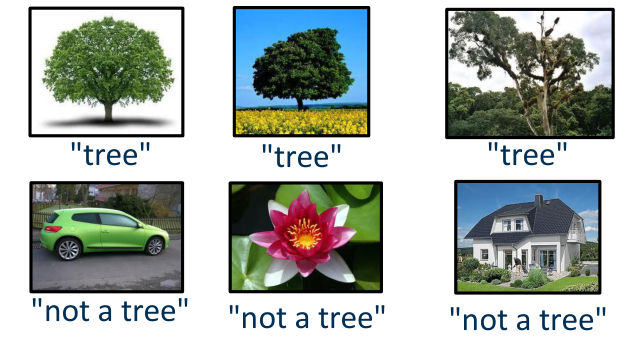
\includegraphics[width=0.65\textwidth,keepaspectratio]{images/thumb_trees_classification.png}\\[0.15cm]
  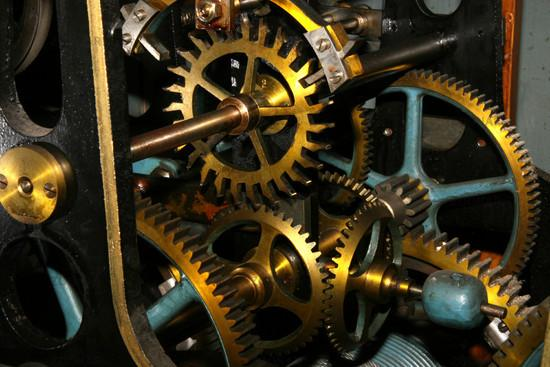
\includegraphics[width=\textwidth,height=3cm,keepaspectratio]{images/img_p48_7_251.jpeg}
\end{center}
\end{column}
\end{columns}
\end{frame}

% Slide 49: K-Nearest-Neighbors Problem
\begin{frame}{الگوریتم نزدیک‌ترین همسایگان (\lr{k-NN})}
\framesubtitle{طرح مسئله پیش‌بینی آب‌وهوا}
\begin{columns}[T,onlytextwidth]
\begin{column}{0.55\textwidth}
\begin{itemize}
  \item \textbf{صورت مسئله:}
  \begin{itemize}
    \item قصد داریم وضعیت هوای فعلی را در نقطه‌ای مشخص (علامت \lr{x}) پیش‌بینی کنیم.
    \item در این نقطه مشخص هیچ ایستگاه هواشناسی مستقر نیست!
    \item چگونه می‌توانیم این پیش‌بینی را با دقت انجام دهیم؟
  \end{itemize}
  \vspace{0.25cm}
  \item \textbf{علائم راهنما:}
  \begin{itemize}
    \item \textbf{قرمز:} آفتابی (\lr{Sunny})
    \item \textbf{آبی:} ابری (\lr{Cloudy})
  \end{itemize}
\end{itemize}
\end{column}
\begin{column}{0.43\textwidth}
\begin{center}
  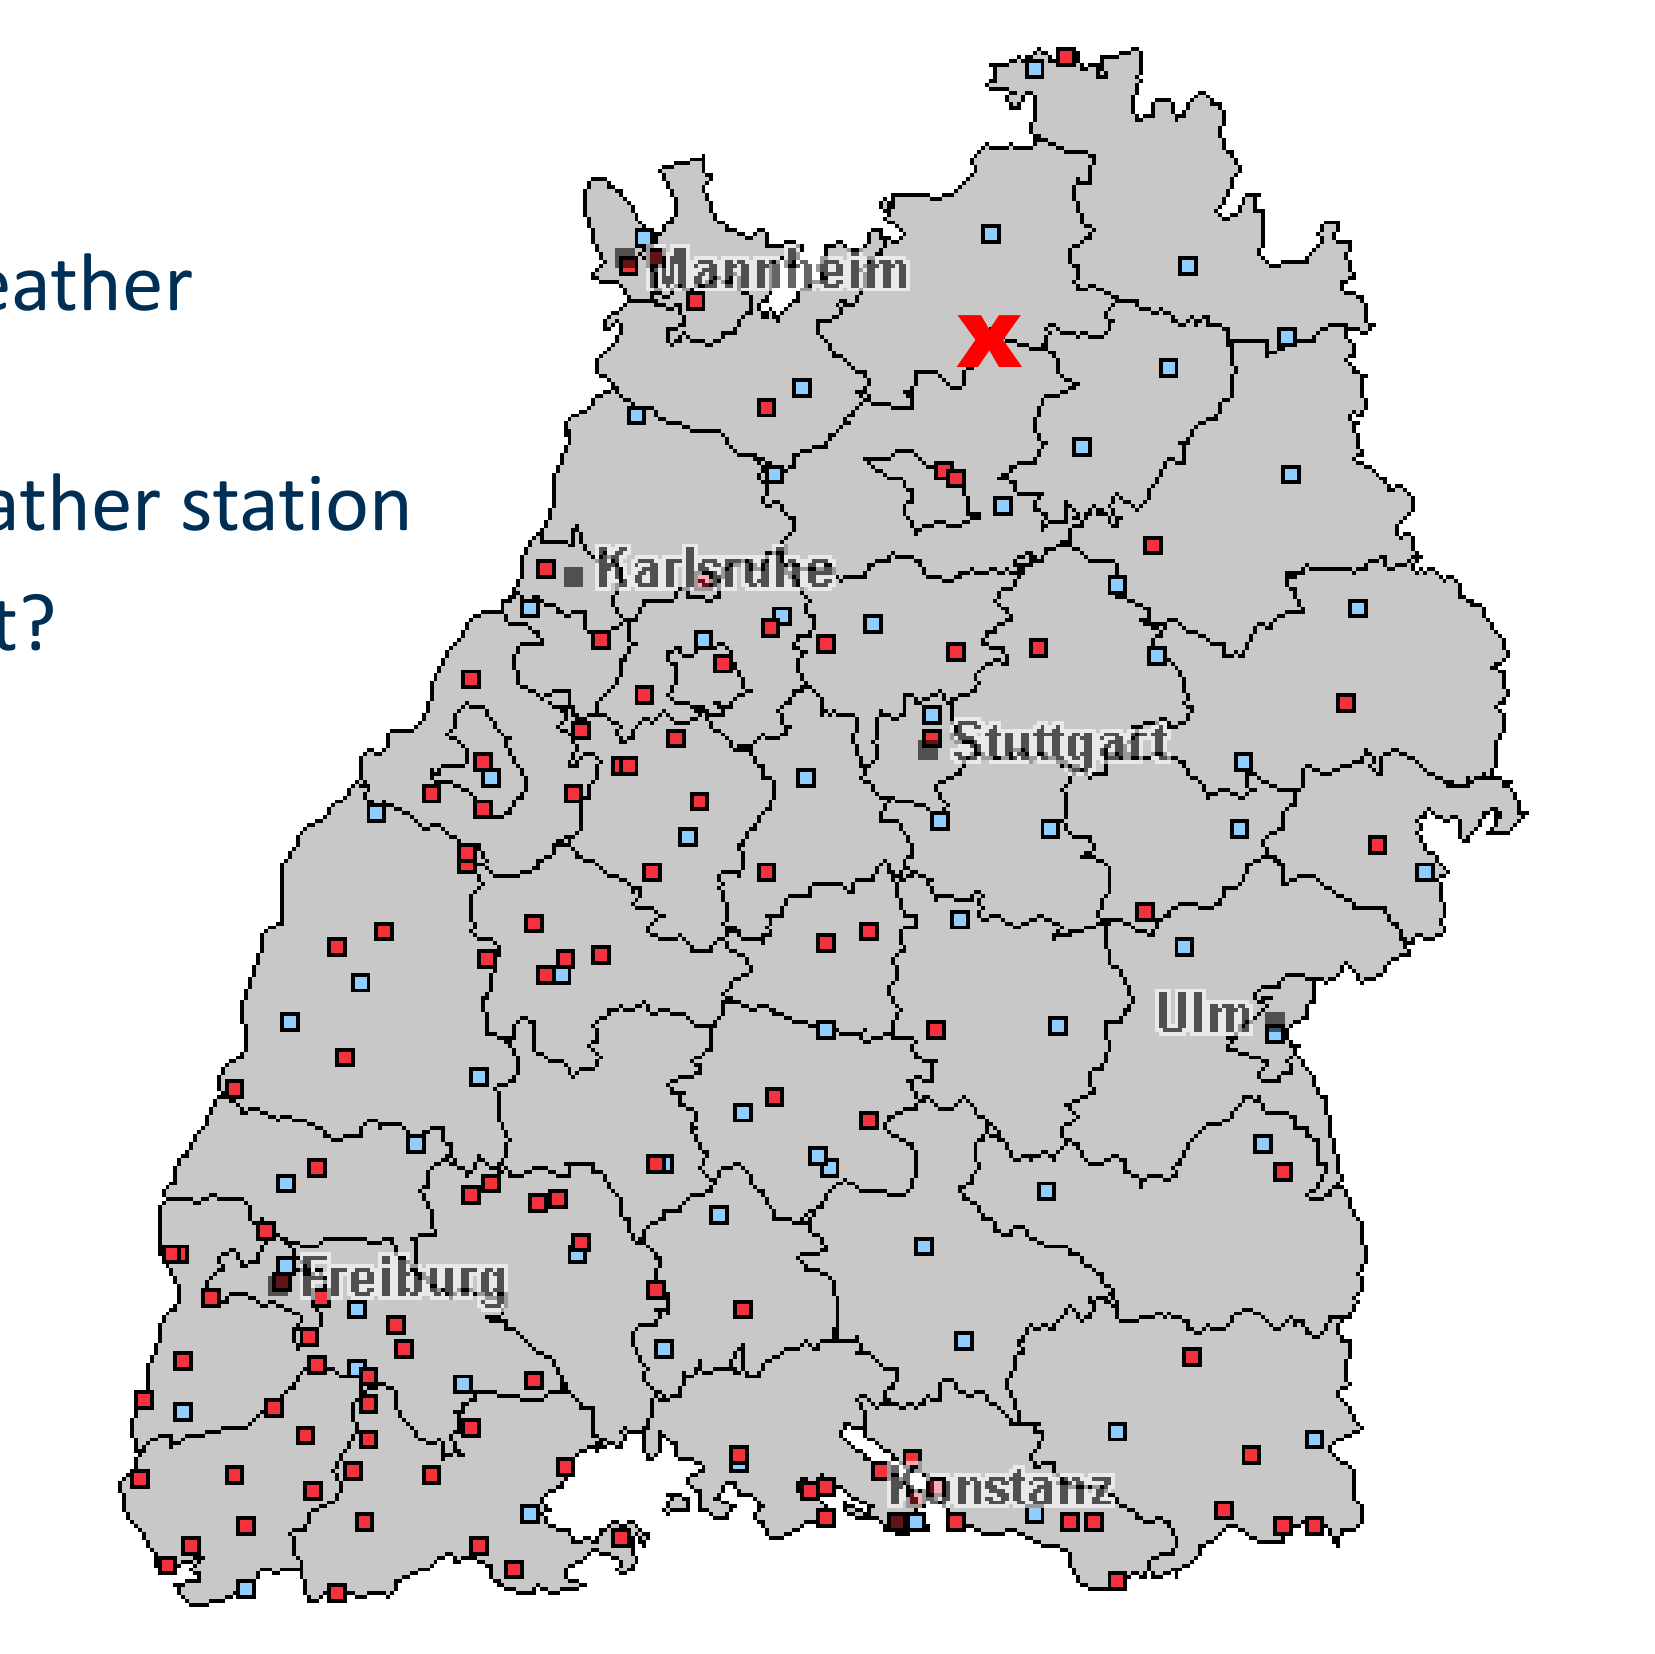
\includegraphics[width=\textwidth,height=4.2cm,keepaspectratio]{images/img_p49_1_258.png}
\end{center}
\end{column}
\end{columns}
\end{frame}

% Slide 50: K-Nearest-Neighbors Idea
\begin{frame}{الگوریتم نزدیک‌ترین همسایگان (\lr{k-NN})}
\framesubtitle{ایده اصلی و شهود حل مسئله}
\begin{columns}[T,onlytextwidth]
\begin{column}{0.55\textwidth}
\begin{itemize}
  \item \textbf{ایده بنیادین:}
  \begin{itemize}
    \item استفاده از میانگین یا رأی اکثریت نزدیک‌ترین ایستگاه‌ها!
  \end{itemize}
  \vspace{0.15cm}
  \item \textbf{مثال عددی با \lr{$k=5$}}
  \begin{itemize}
    \item \lr{2} ایستگاه آفتابی (قرمز)
    \item \lr{3} ایستگاه ابری (آبی)
    \item $\Rightarrow$ \textbf{نتیجه پیش‌بینی: ابری (\lr{Cloudy})}
  \end{itemize}
  \vspace{0.15cm}
  \item \textbf{نام‌گذاری روش:}
  \begin{itemize}
    \item \lr{$k$} تعداد همسایگان بررسی‌شده است (\lr{$k=5$}).
    \item «نزدیکی» دلالت بر مجاورت در فضای ویژگی‌ها (اینجا فاصله جغرافیایی) دارد.
  \end{itemize}
\end{itemize}
\end{column}
\begin{column}{0.43\textwidth}
\begin{center}
  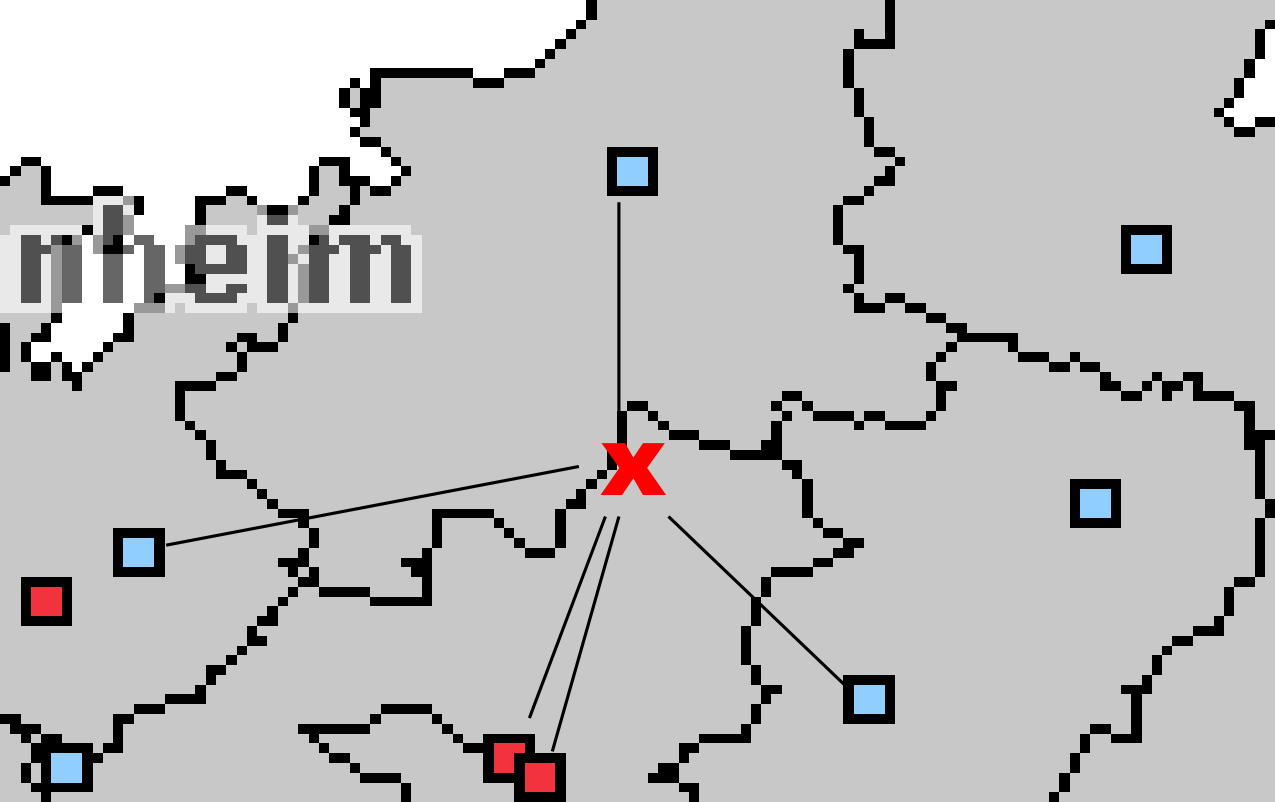
\includegraphics[width=\textwidth,height=4.2cm,keepaspectratio]{images/img_p50_1_261.png}
\end{center}
\end{column}
\end{columns}
\end{frame}

% Slide 51: K-NN Classifier Requirements
\begin{frame}{سه پیش‌نیاز اصلی دسته‌بند \lr{k-NN}}
\begin{columns}[c,onlytextwidth]
\begin{column}{0.42\textwidth}
\begin{center}
  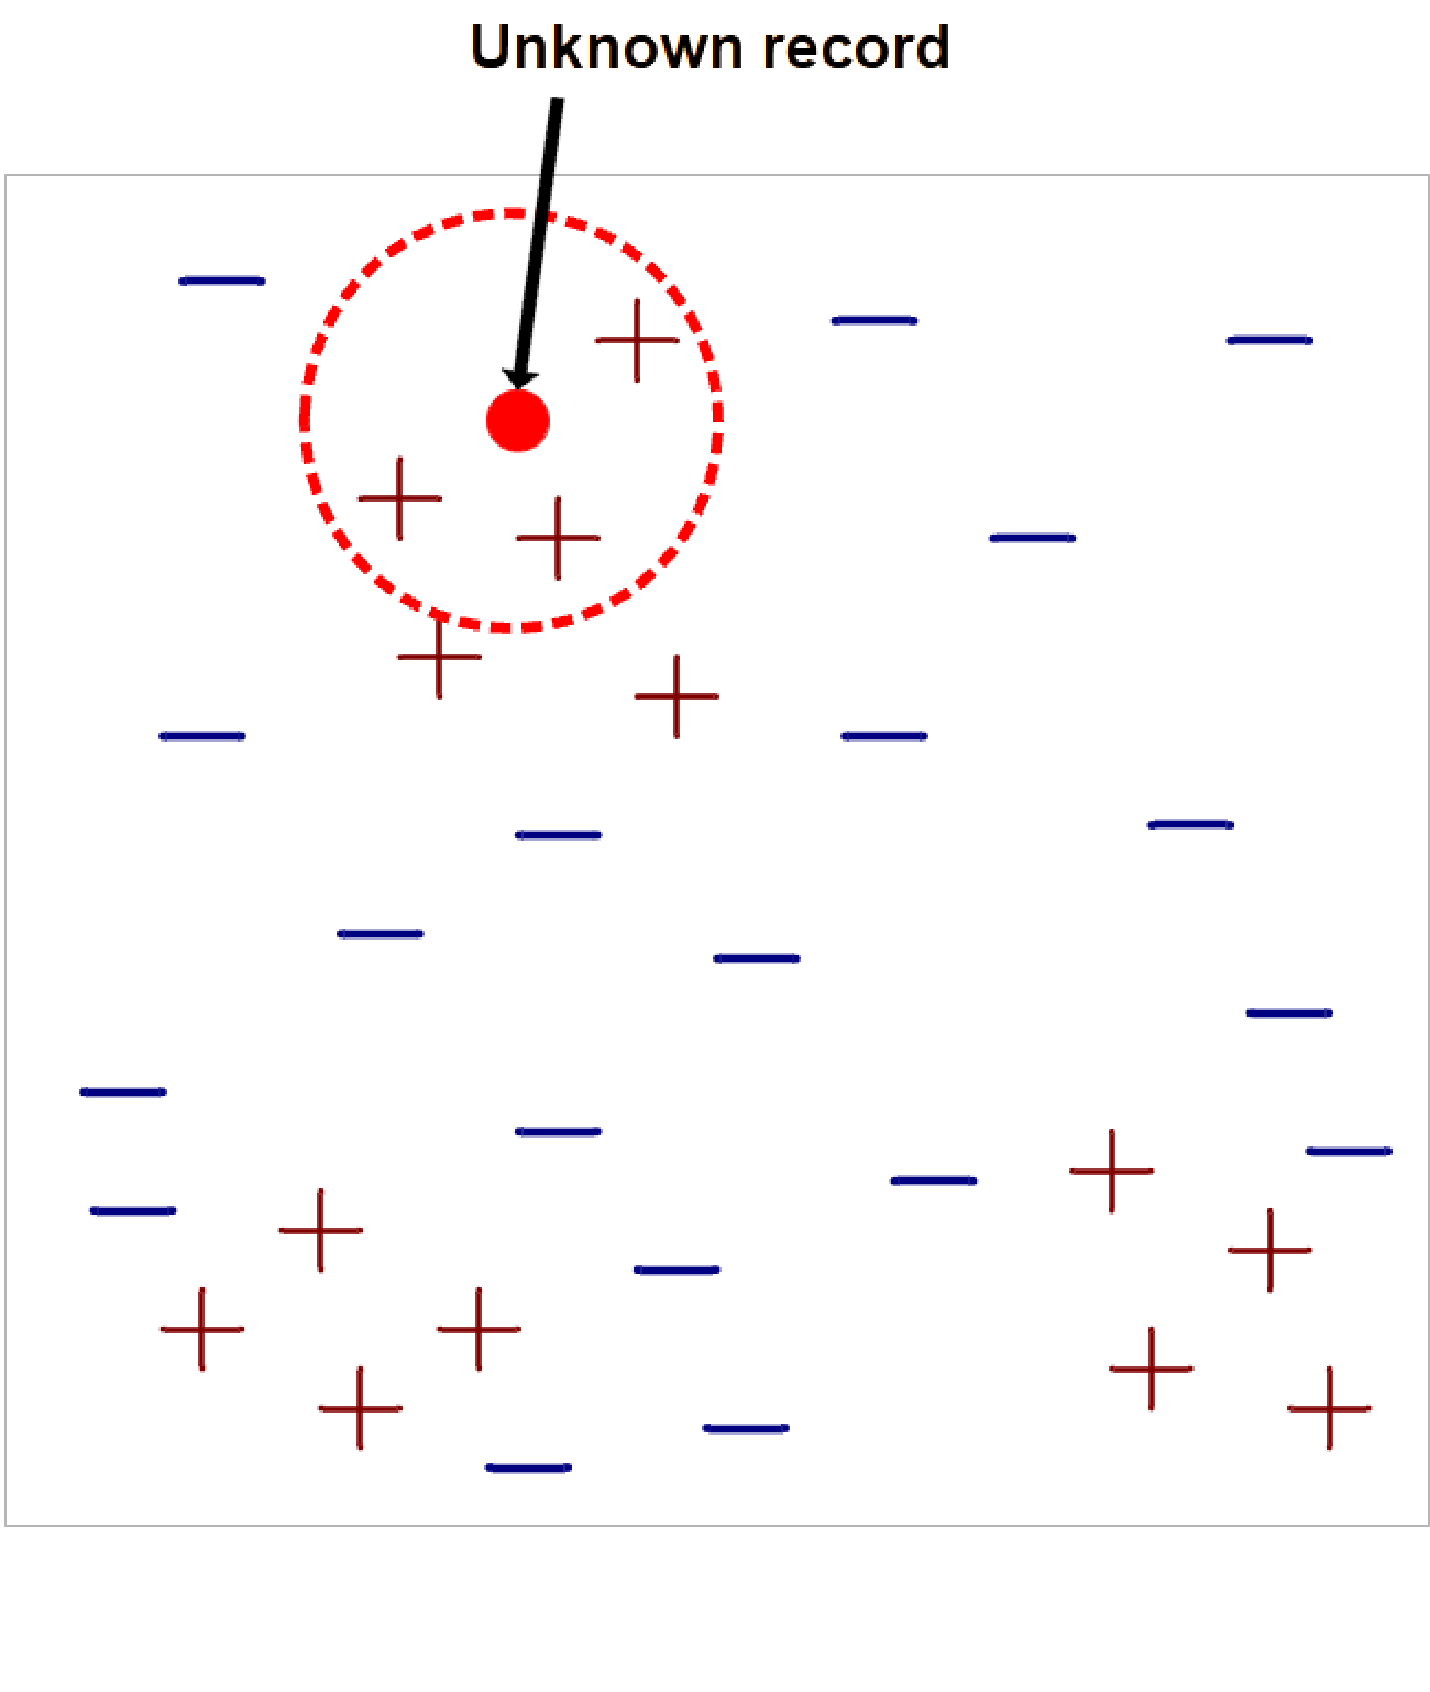
\includegraphics[width=\textwidth,height=4cm,keepaspectratio]{images/img_p51_1_264.png}
\end{center}
\end{column}
\begin{column}{0.55\textwidth}
\begin{itemize}
  \item \textbf{برای پیاده‌سازی دسته‌بند \lr{k-NN} به سه مؤلفه نیاز است:}
  \begin{enumerate}
    \item \textbf{مجموعه رکوردهای آموزشی} -- داده‌های ذخیره‌شده با برچسب‌های معتبر کلاس
    \item \textbf{معیار فاصله} (\lr{Distance Metric}) -- تابعی برای محاسبه فاصله بین رکوردها
    \item \textbf{تعیین پارامتر} \lr{$k$} -- تعداد نزدیک‌ترین همسایگان برای رأی‌گیری
  \end{enumerate}
\end{itemize}
\end{column}
\end{columns}
\end{frame}

% Slide 52: K-NN Classifier Algorithm
\begin{frame}{مراحل الگوریتم دسته‌بندی \lr{k-NN}}
\begin{columns}[c,onlytextwidth]
\begin{column}{0.42\textwidth}
\begin{center}
  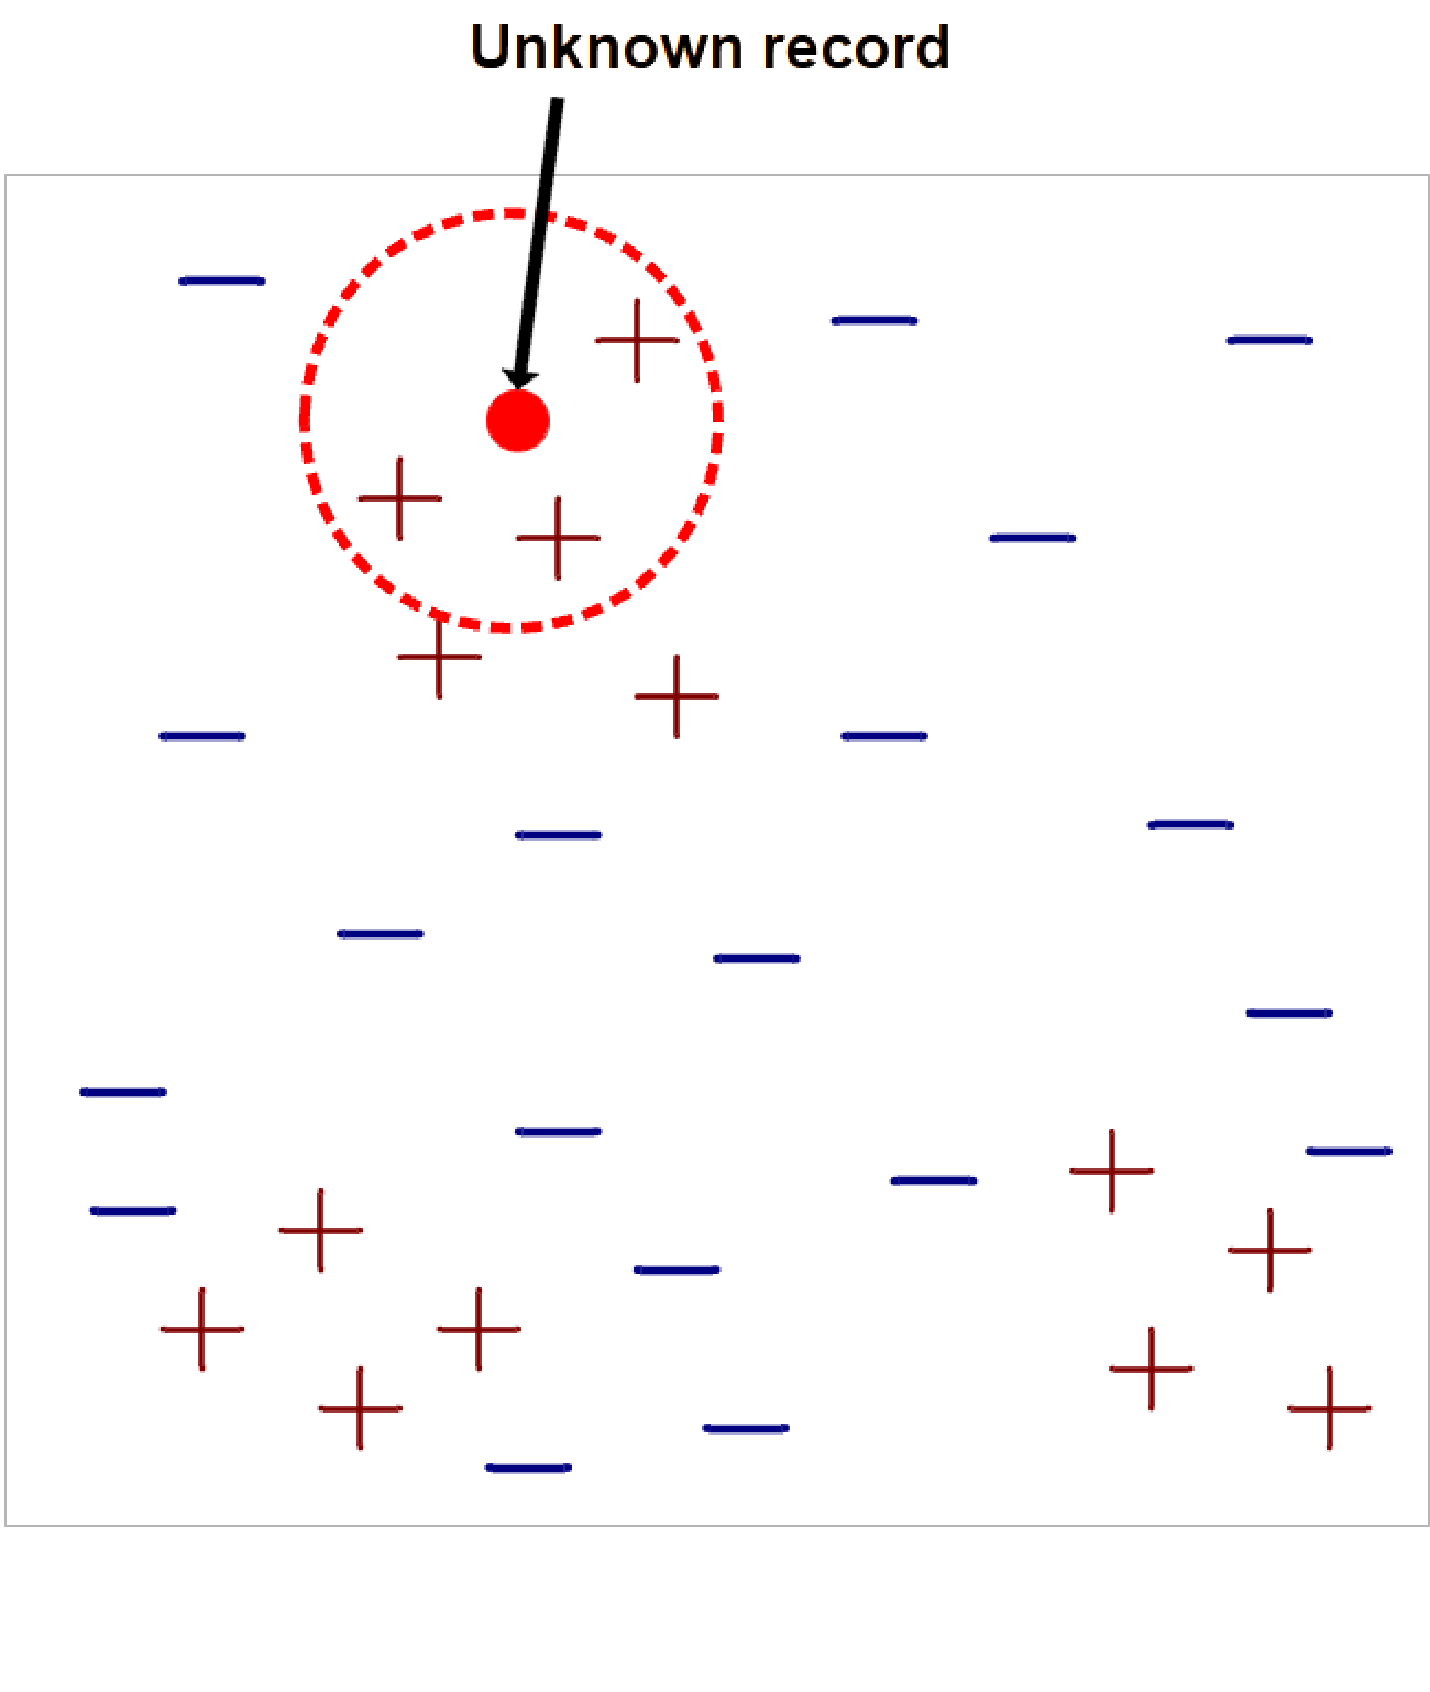
\includegraphics[width=\textwidth,height=4cm,keepaspectratio]{images/img_p51_1_264.png}
\end{center}
\end{column}
\begin{column}{0.55\textwidth}
\begin{enumerate}
  \item محاسبه فاصله نقطه جدید تا تمام نمونه‌های آموزشی
  \item مرتب‌سازی و انتخاب \lr{$k$} نمونه دارای کمترین فاصله
  \item برچسب‌گذاری نقطه جدید با برچسب‌های این \lr{$k$} همسایه:
  \begin{itemize}
    \item \textbf{رأی اکثریت ساده} (\lr{Majority Vote})
    \item \textbf{رأی وزن‌دار با معکوس فاصله} (\lr{Distance-Weighted})
  \end{itemize}
\end{enumerate}
\end{column}
\end{columns}
\end{frame}

% Slide 53: Examples of K-Nearest Neighbors
\begin{frame}{نمونه‌هایی از انتخاب همسایگان در الگوریتم \lr{k-NN}}
\begin{itemize}
  \item \textbf{تعریف همسایگی:} همسایگان نزدیک برای یک نمونه داده \lr{$x$}، نقاطی از داده‌ها هستند که کمترین فاصله را تا \lr{$x$} دارند.
\end{itemize}
\begin{center}
  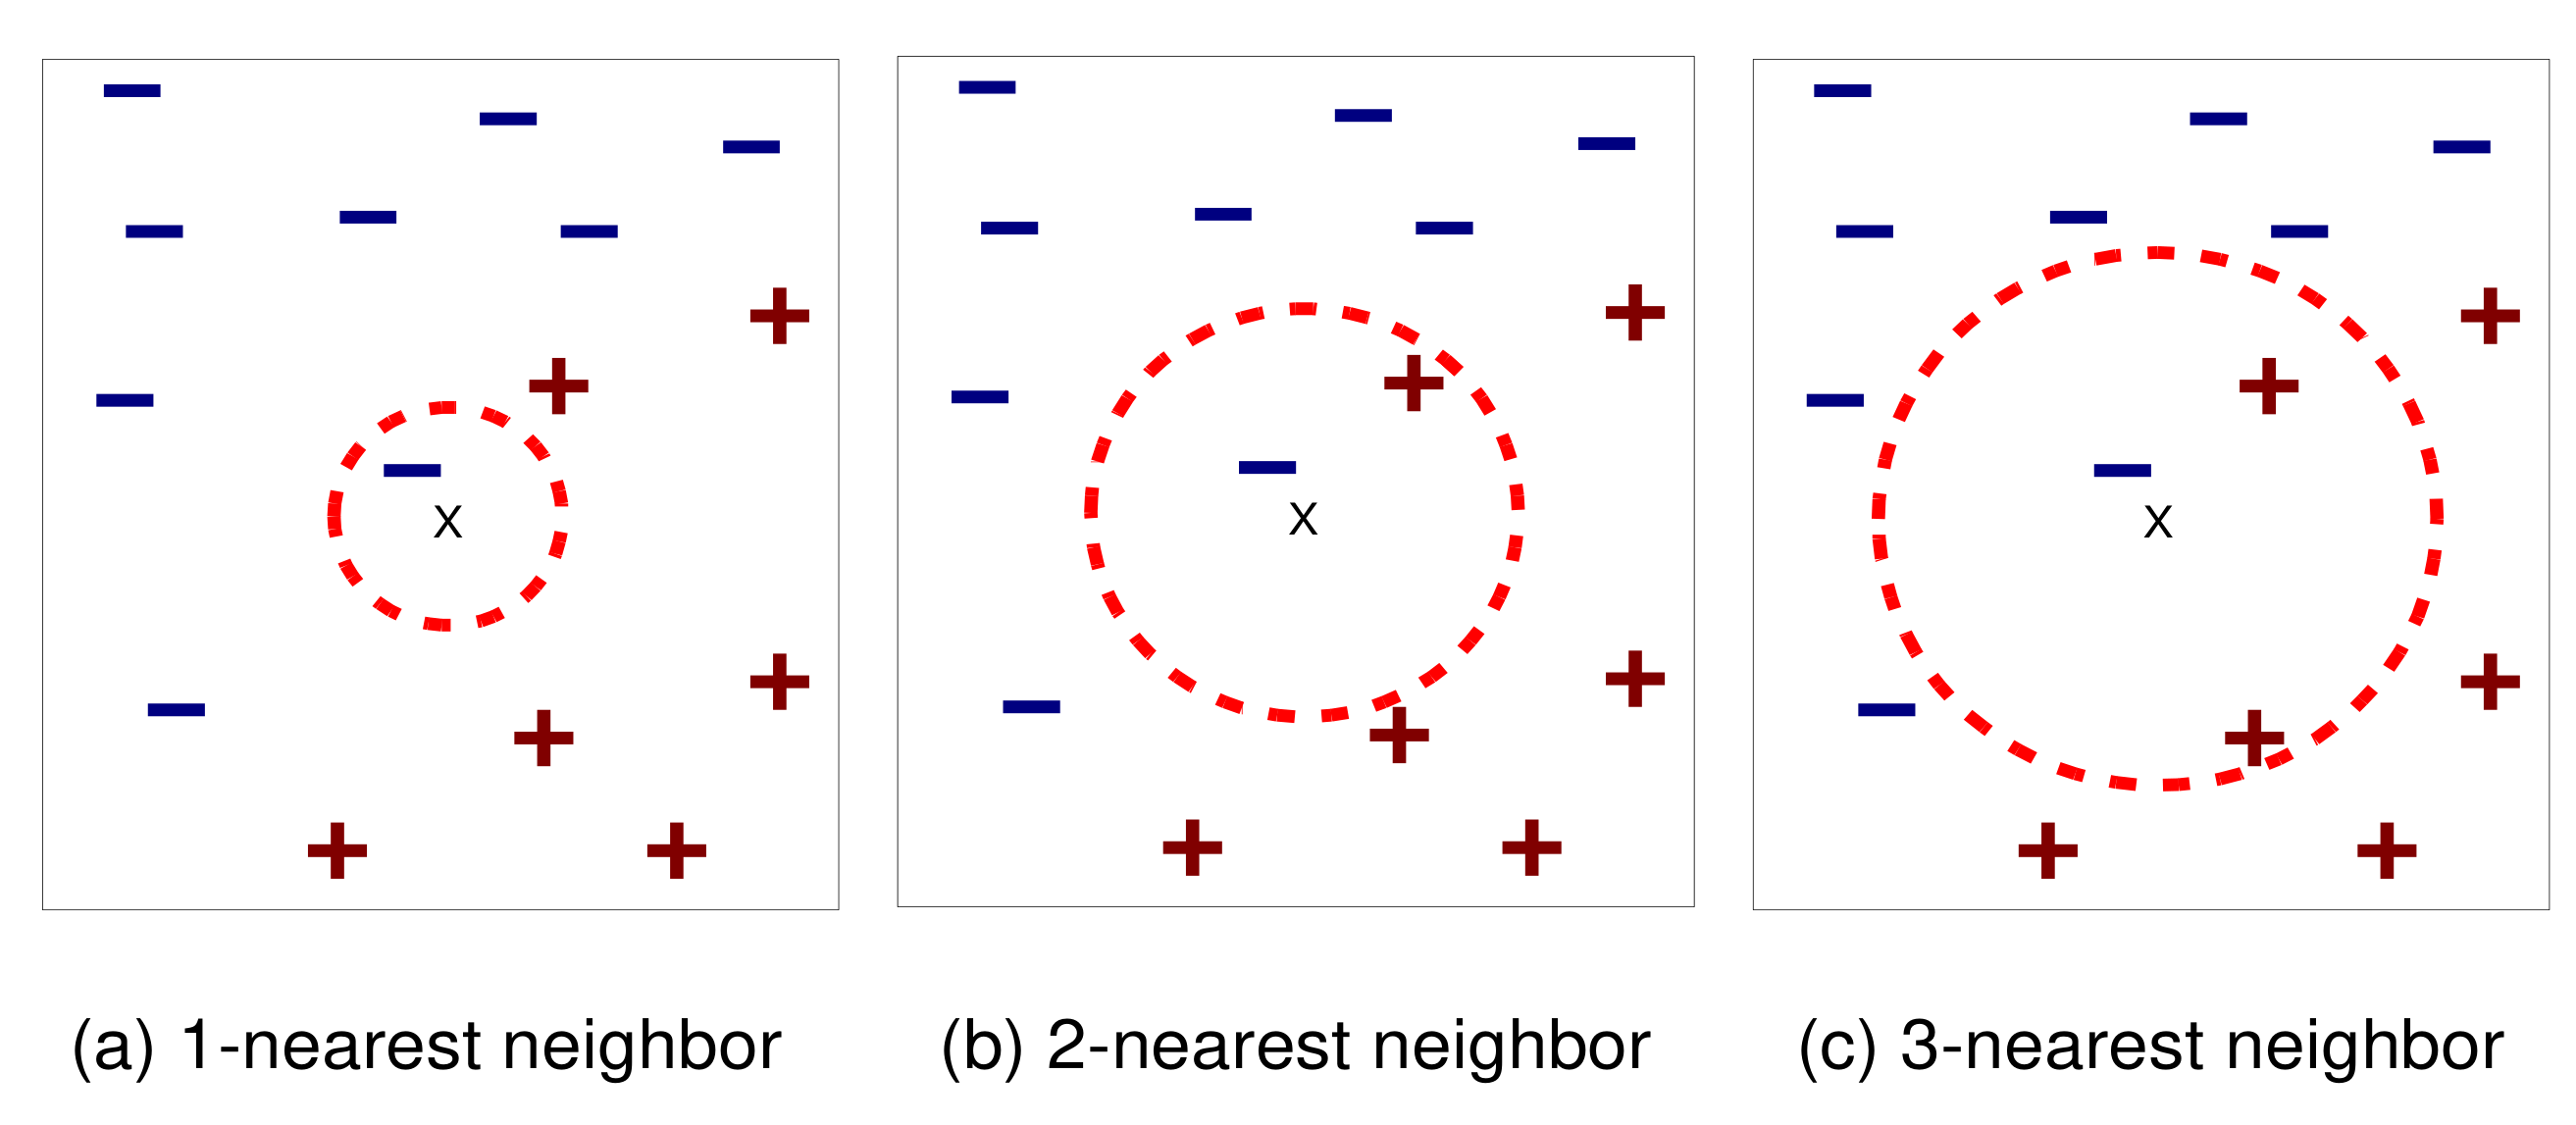
\includegraphics[width=0.88\textwidth,height=4.2cm,keepaspectratio]{images/diagram_p53_knn_examples.png}
\end{center}
\end{frame}

% Slide 54: Choosing a Good Value for K
\begin{frame}{انتخاب مقدار بهینه برای پارامتر \lr{k}}
\begin{itemize}
  \item \textbf{اگر مقدار \lr{$k$} بسیار کوچک باشد (مانند \lr{$k=1$}) --} مدل به‌شدت به نویزها و داده‌های پرت حساس شده و دچار بیش‌برازش (\lr{Overfitting}) می‌گردد.
  \item \textbf{اگر مقدار \lr{$k$} بسیار بزرگ باشد:} ناحیه همسایگی گسترده شده و نقاطی از کلاس‌های دیگر در تصمیم اثر می‌گذارند.
\end{itemize}
\begin{center}
  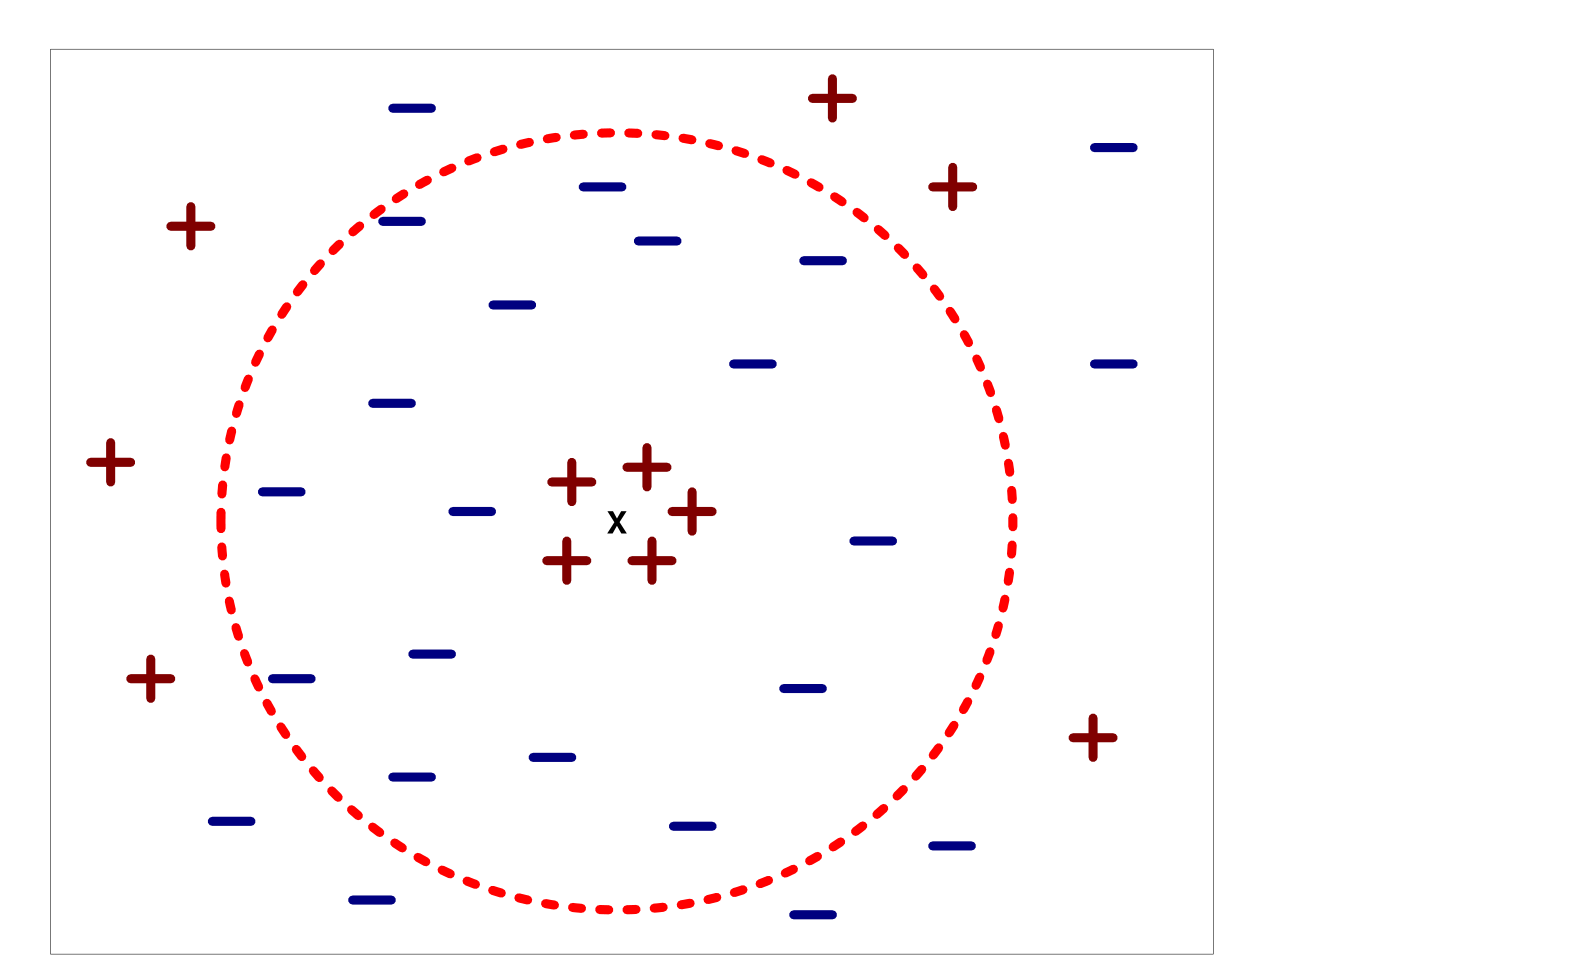
\includegraphics[width=0.68\textwidth,height=3cm,keepaspectratio]{images/diagram_p54_knn_choice.png}\\[0.1cm]
  {\small\textbf{قاعده تجربی} (\lr{Rule of Thumb}) -- ارزیابی مقادیر \lr{$k$} در بازهٔ \lr{1} تا \lr{20} به کمک اعتبارسنجی متقاطع.}
\end{center}
\end{frame}

% Slide 55: Discussion of K-NN Classification
\begin{frame}{تحلیل و ارزیابی دسته‌بند \lr{k-NN}}
\begin{itemize}
  \item \textbf{نقاط قوت و دقت بالا:}
  \begin{itemize}
    \item در بسیاری از مسائل دسته‌بندی عملکرد بسیار چشمگیری دارد (مانند بازشناسی نوری حروف \lr{OCR}).
    \item قادر است مرزهای تصمیم‌گیری پیچیده و غیرموازی با محورها را به‌خوبی مدل‌سازی کند (برخلاف درخت‌های تصمیم ساده).
  \end{itemize}
  \vspace{0.25cm}
  \item \textbf{چالش‌ها و ملاحظات عملی:}
  \begin{itemize}
    \item \textbf{سرعت کند در زمان آزمون} (\lr{Lazy Learner}) -- مدل‌سازی قبلی ندارد و در لحظه پیش‌بینی باید با تمام داده‌های آموزشی مقایسه شود.
    \item \textbf{حساسیت به مقیاس و فاصله:} نیاز به نرمال‌سازی متغیرها و انتخاب وزن مناسب برای ویژگی‌ها.
  \end{itemize}
\end{itemize}
\end{frame}

% Slide 56: Decision Boundaries of k-NN (k=1)
\begin{frame}{مرزهای تصمیم‌گیری در دسته‌بند \lr{k-NN} (حالت \lr{$k=1$})}
\begin{itemize}
  \item در حالت \lr{$k=1$}، تک‌تک نقاط نویز مستقیماً مرزهای تصمیم‌گیری را تغییر داده و ساختار پیچیده ایجاد می‌کنند:
\end{itemize}
\begin{center}
  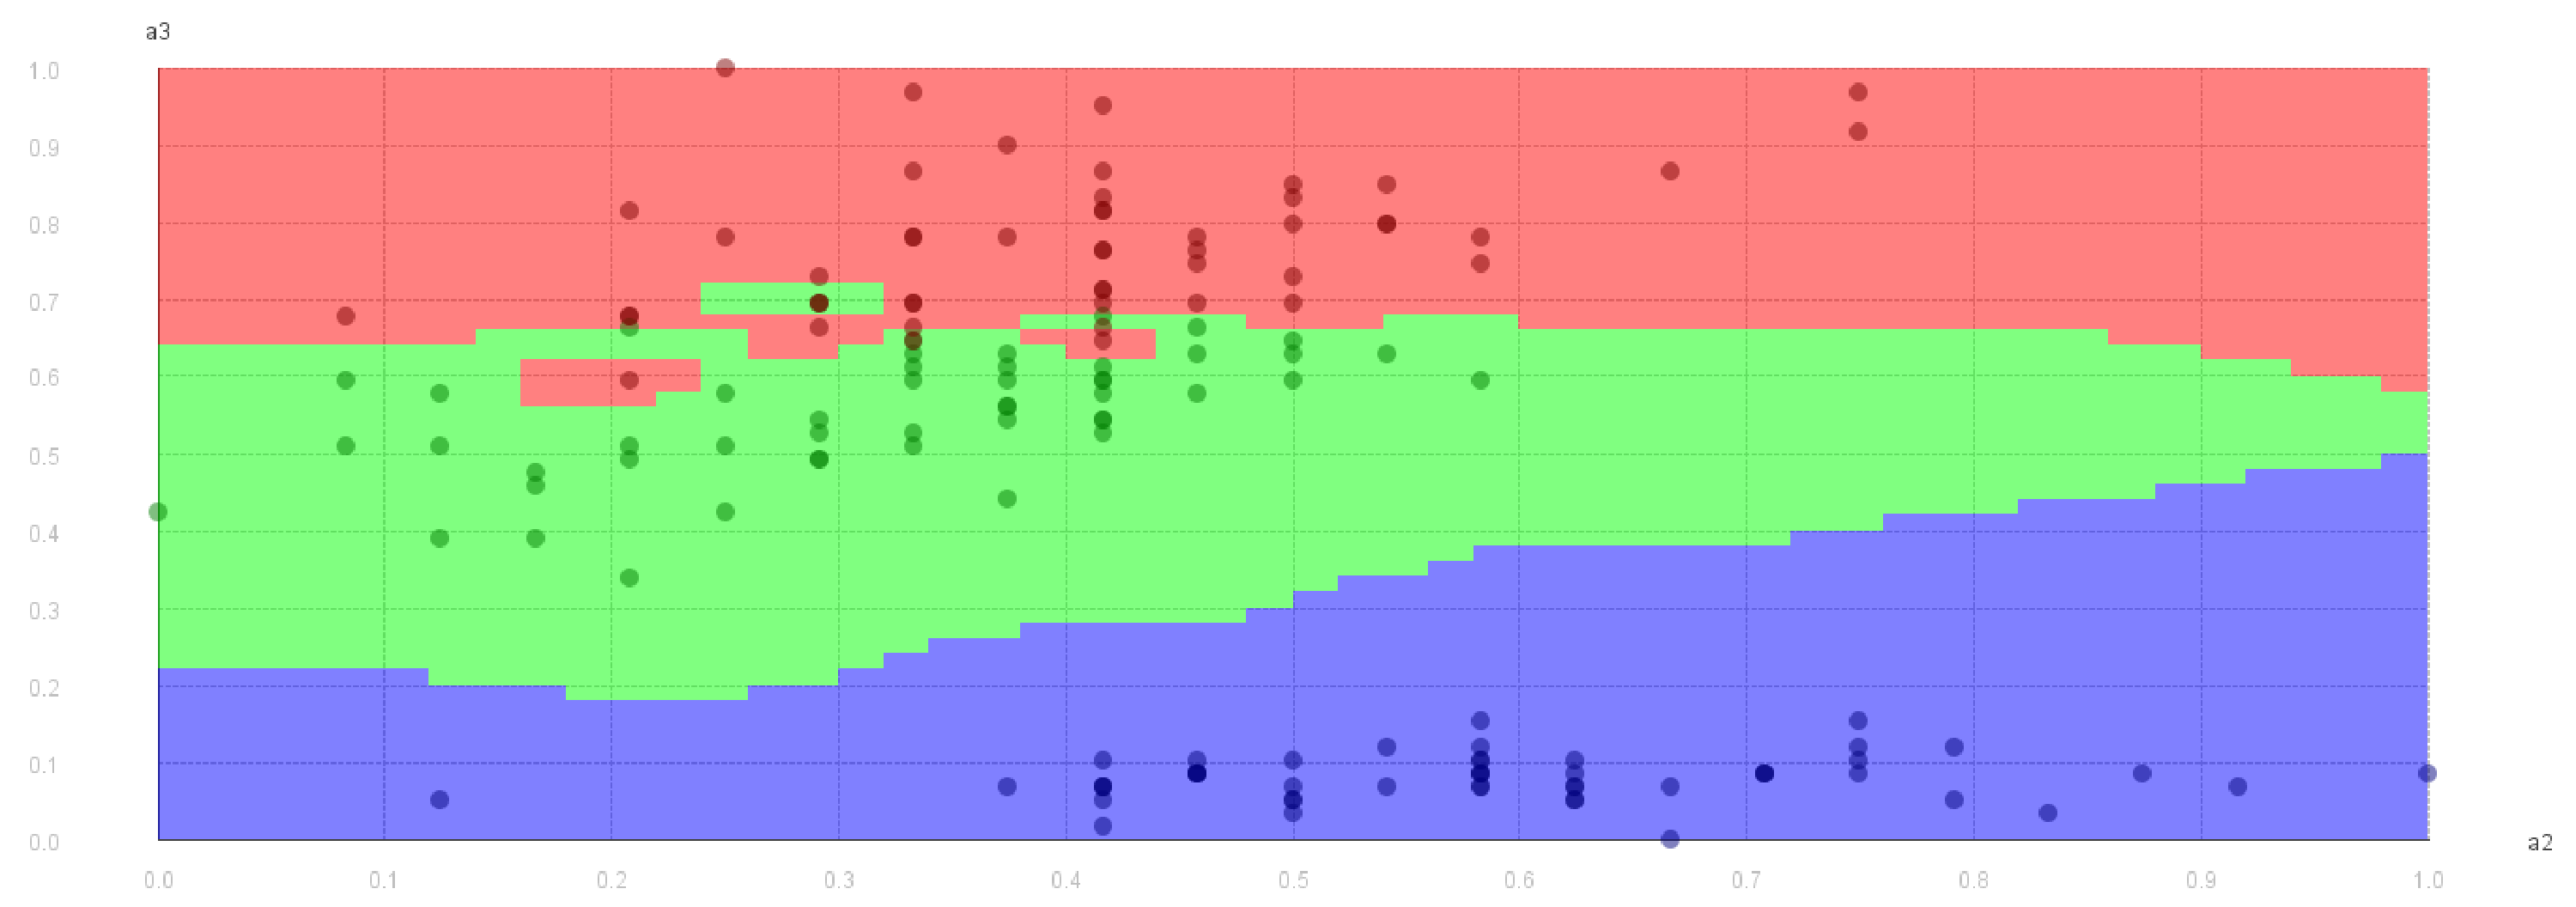
\includegraphics[width=0.92\textwidth,height=4.1cm,keepaspectratio]{images/img_p56_1_278.png}
\end{center}
\end{frame}

% Slide 57: Decision Boundaries of k-NN (k=3)
\begin{frame}{مرزهای تصمیم‌گیری در دسته‌بند \lr{k-NN} (حالت \lr{$k=3$})}
\begin{itemize}
  \item با افزایش تعداد همسایگان به \lr{$k=3$}، مرزها هموارتر شده و اثر نویزها تا حد زیادی کاهش می‌یابد:
\end{itemize}
\begin{center}
  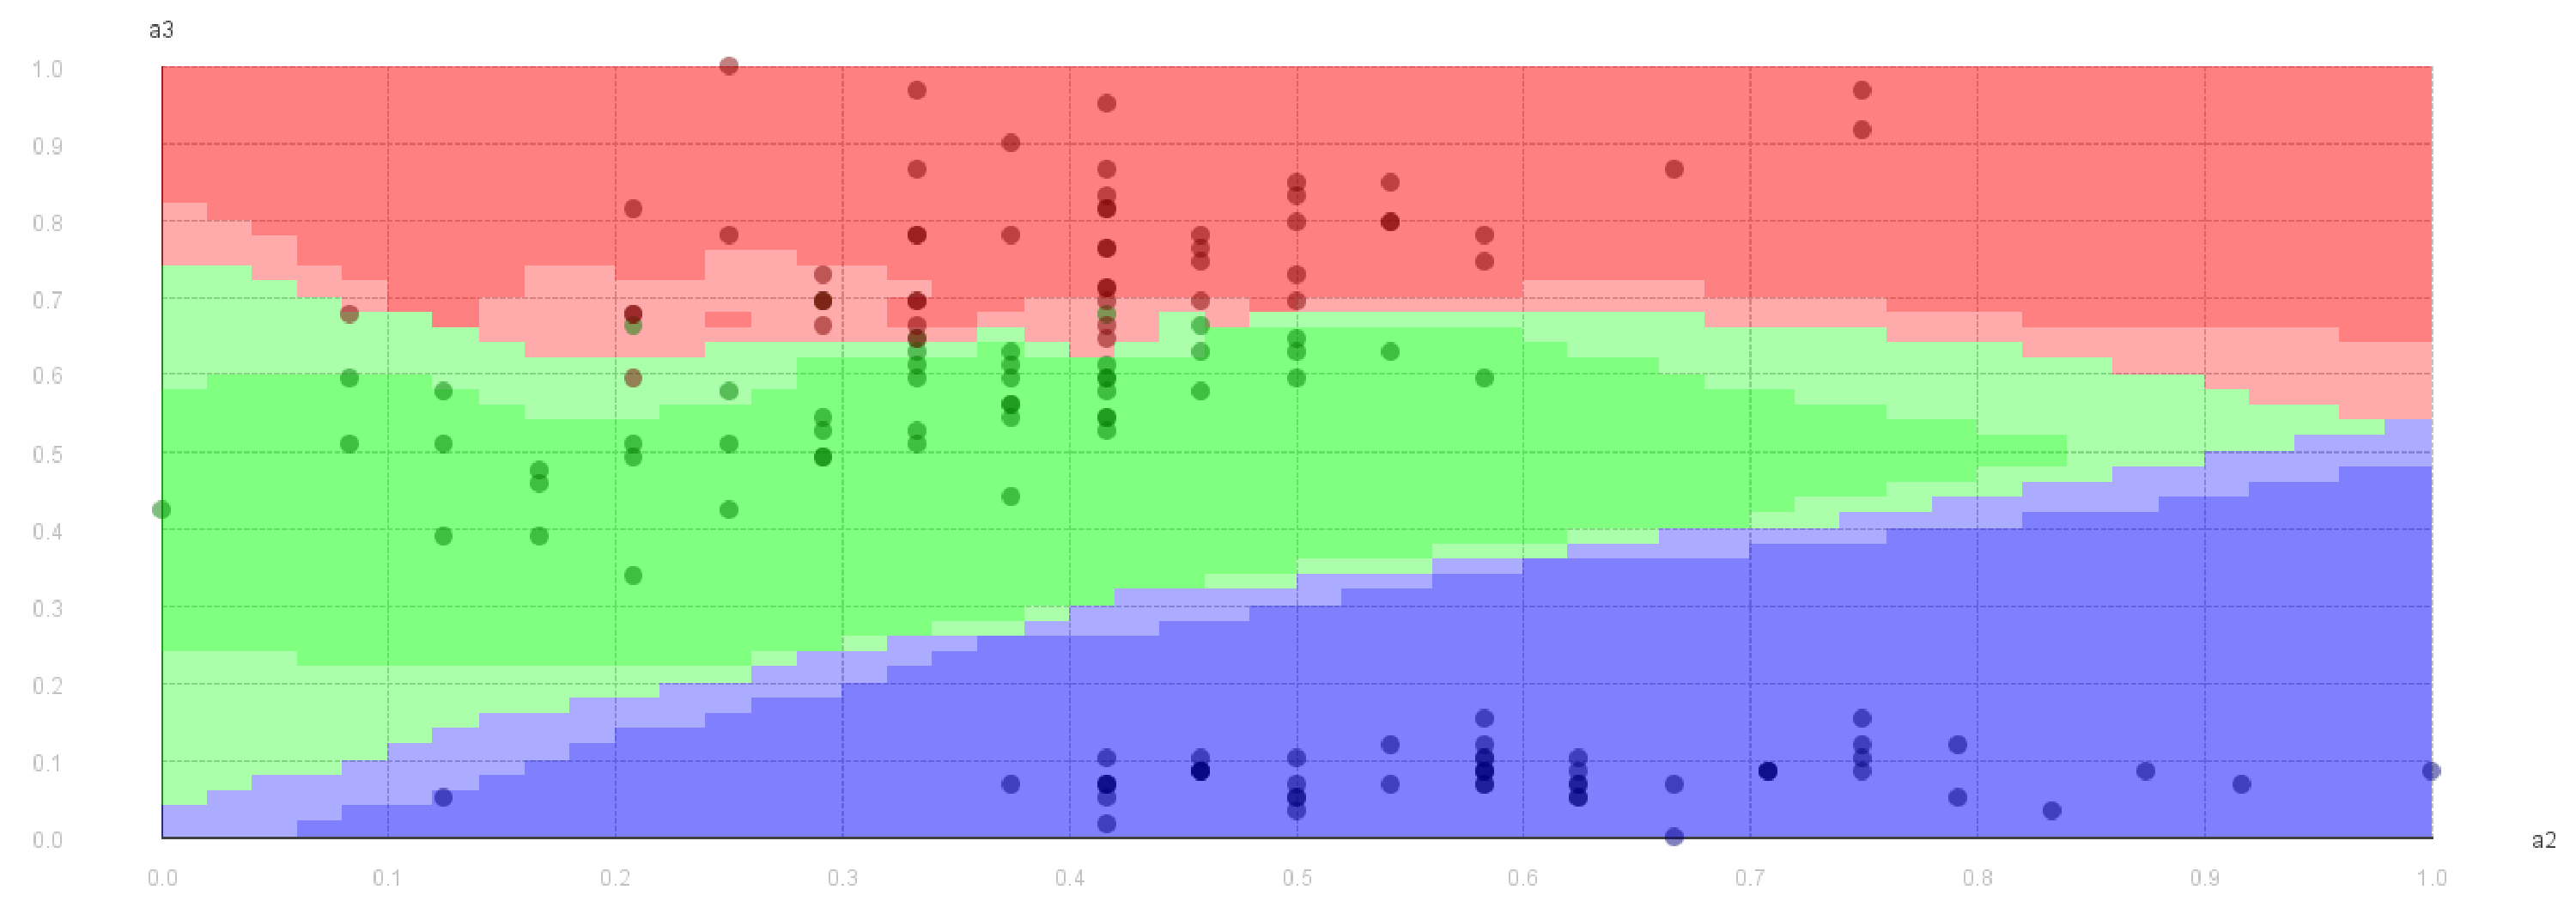
\includegraphics[width=0.92\textwidth,height=4.1cm,keepaspectratio]{images/img_p57_1_281.png}
\end{center}
\end{frame}

% Slide 58: What You Will Learn in This Lecture
\begin{frame}{آنچه در این درس خواهید آموخت}
\begin{columns}[T,onlytextwidth]
\begin{column}{0.6\textwidth}
\begin{itemize}
  \item \textbf{وظایف اصلی و رایج داده‌کاوی:}
  \begin{itemize}
    \item پیش‌پردازش، پاک‌سازی و مهندسی داده‌ها
    \item الگوریتم‌های دسته‌بندی و پیش‌بینی
    \item تکنیک‌های خوشه‌بندی و تحلیل بدون نظارت
    \item کاوش قوانین وابستگی و سبد خرید
  \end{itemize}
  \vspace{0.2cm}
  \item \textbf{مهارت‌های عملی و نظری:}
  \begin{itemize}
    \item درک ریاضی و منطق پشت الگوریتم‌ها
    \item نحوه و شرایط کاربرد هر متد در مسائل واقعی
    \item تفسیر درست و علمی خروجی‌ها و شاخص‌های ارزیابی
  \end{itemize}
\end{itemize}
\end{column}
\begin{column}{0.38\textwidth}
\begin{center}
  
\includegraphics[width=\textwidth,height=4.2cm,keepaspectratio]{images/img_p58_1_284.png}
\end{center}
\end{column}
\end{columns}
\end{frame}

% Slide 59: Thank you
\begin{frame}{پایان جلسه و گام‌های بعدی}
\begin{center}
  \vspace{1.2cm}
  {\fontsize{22}{26}\selectfont\color{mannheimblue}\textbf{با سپاس از توجه شما}}\\[0.6cm]
  {\fontsize{14}{18}\selectfont\color{mannheimgold}\textbf{آیا پرسش یا ابهامی باقی مانده است؟}}\\[0.8cm]
  {\fontsize{10}{12}\selectfont\color{subgray}در جلسه آینده: مبانی آماده‌سازی، کاوش و پیش‌پردازش داده‌ها}\\[0.4cm]
  
\includegraphics[height=1cm]{images/mannheim_logo.png}
\end{center}
\end{frame}
